\clearpage
\chapter{Norton Guide: \RU{простейшее XOR-шифрование}\EN{simplest possible XOR encryption}}

\EN{Norton Guide\footnote{\href{http://go.yurichev.com/17116}{wikipedia}} was popular in MS-DOS epoch, it was resident program working as hypertext reference.}
\RU{Norton Guide\footnote{\href{http://go.yurichev.com/17116}{wikipedia}} был популярен во времена MS-DOS, это была резидентная программа, работающая как
гипертекстовый справочник.}

\EN{Norton Guide databases are files with .ng extensions, contents of which looks encrypted:}
\RU{Базы данных Norton Guide это файлы с расширением .ng, содержимое которых выглядит как зашифрованное:}

\begin{figure}[H]
\centering
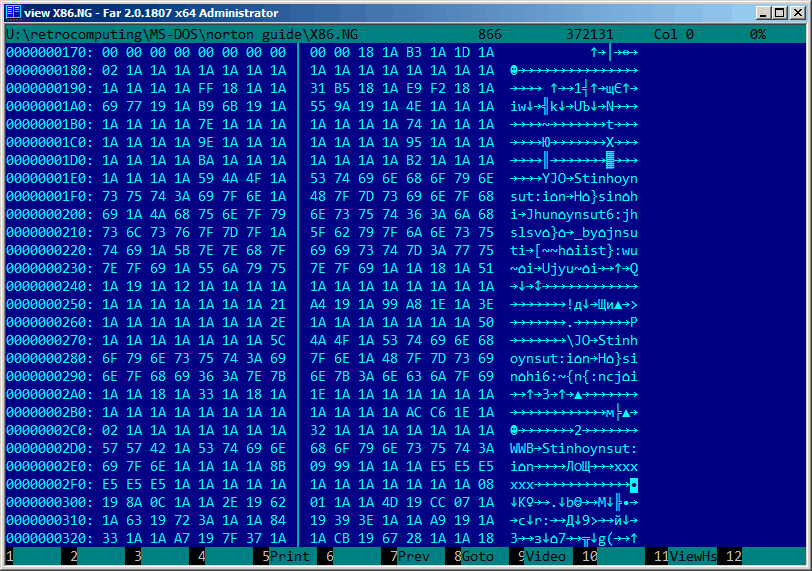
\includegraphics[scale=\FigScale]{ff/ng/ng1.png}
\caption{\RU{Очень типичный вид}\EN{Very typical look}}
\end{figure}

\EN{Why did I wrote it's encrypted but not compressed?}
\RU{Почему я написал что зашифрованное а не сжатое? }
\EN{We see that 0x1A byte (looking like ``$\rightarrow$'') is ocurring so often, it would not be possible in compressed file.}
\RU{Мы видим как слишком часто попадается байт 0x1A (который выглядит как ``$\rightarrow$''), в сжатом файле такого не было бы никогда.}
\EN{We also see long parts consisting only on latin letters, and they looks like strings in unknown
language.}
\RU{Во вторых, мы видим длинные части состоящие только из латинских букв, они выглядят как строки
на незнакомом языке.}

\clearpage
\EN{Since 0x1A byte ocurring so often, we can try to decrypt the file, assuming that it's encrypted
by simplest XOR-encryption.}
\RU{Из-за того что байт 0x1A слишком часто встречается, мы можем попробовать расшифровать файл, полагая
что он зашифрован простейшим XOR-шифрованием.}
\EN{Let's apply XOR with 0x1A constant to each byte in Hiew and we will see familiar English text strings:}
\RU{Применяем XOR с константой 0x1A к каждому байту в Hiew и мы видим знакомые текстовые строки на английском:}

\begin{figure}[H]
\centering
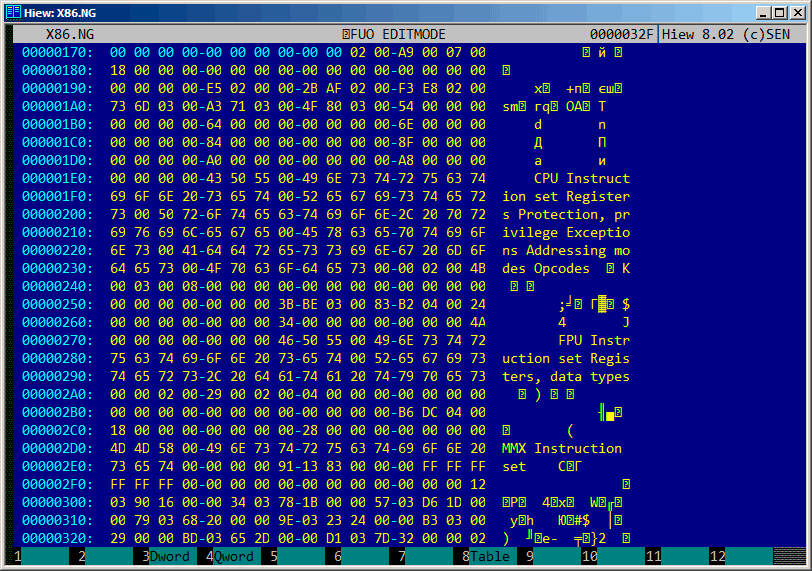
\includegraphics[scale=\FigScale]{ff/ng/ng2.png}
\caption{Hiew \RU{применение XOR с 0x1A}\EN{XORing with 0x1A}}
\end{figure}

\EN{XOR-encryption with one single constant byte is simplest possible encryption method, which is, nevertheless,
encountering sometimes.}
\RU{XOR-шифрование с одним константным байтом это самый простой способ шифрования, который, тем не менее, иногда
встречается.}

\EN{Now we understand why 0x1A byte was ocurring so often: because there are so much zero bytes and they
were replaced by 0x1A in encrypted form.}
\RU{Теперь понятно почему байт 0x1A так часто встречался: потому что в файле очень много нулевых байт 
и в зашифрованном виде они везде были заменены на 0x1A.}

\EN{But the constant might be different}\RU{Но эта константа могла быть другой}.
\EN{In this case, we could try each constant in 0..255 range and look for something familiar in decrypted
file. 256 is not so much.}
\RU{В таком случае, можно было бы попробовать перебрать все 256 комбинаций, и посмотреть содержимое ``на глаз'', 
а 256 --- это совсем немного.}

\EN{More about Norton Guide file format:}
\RU{Больше о формате файлов Norton Guide:} \url{http://go.yurichev.com/17317}.
